\documentclass{article}
%\usepackage[english]{babel}%
\usepackage{graphicx}
\usepackage{tabulary}
\usepackage{tabularx}
\usepackage[table,xcdraw]{xcolor}
\usepackage{pdflscape}
%\usepackage{gensymb}
\usepackage{lastpage}
\usepackage{multirow}
\usepackage{xcolor}
\usepackage{cancel}
\usepackage{amsmath}
\usepackage[table]{xcolor}
\usepackage{fixltx2e}
\usepackage[T1]{fontenc}
\usepackage[utf8]{inputenc}
\usepackage{ifthen}
\usepackage{fancyhdr}
\usepackage[utf8]{inputenc}
\usepackage{tikz}
\usepackage[document]{ragged2e}
\usepackage[margin=1in,top=1.2in,headheight=57pt,headsep=0.1in]
{geometry}
\usepackage{ifthen}
\usepackage{fancyhdr}
\everymath{\displaystyle}
\usepackage[document]{ragged2e}
\usepackage{fancyhdr}
\usepackage{mathabx}
\usepackage{textcomp,mathcomp}
\usepackage[shortlabels]{enumitem}
\everymath{\displaystyle}
\linespread{2}%controls the spacing between lines. Bigger fractions means crowded lines%
\linespread{1.3}%controls the spacing between lines. Bigger fractions means crowded lines%
\pagestyle{fancy}
\setlength{\headheight}{56.2pt}
\usepackage{soul}
\usepackage{siunitx}

%\usepackage{textcomp}
\usetikzlibrary{shapes.multipart, shapes.geometric, arrows}
\usetikzlibrary{calc, decorations.markings}
\usetikzlibrary{arrows.meta}
\usetikzlibrary{shapes,snakes}
\usetikzlibrary{quotes,angles, positioning}
%\chead{\ifthenelse{\value{page}=1}{
\includegraphics[scale=0.3]{BassettCTCLogo}}}
%\rhead{\ifthenelse{\value{page}=1}{Final Exam}{}}
%\lhead{\ifthenelse{\value{page}=1}{Water Treatment - Oct-Dec 2022}{\textbf Final Exam}}
%\rfoot{\ifthenelse{\value{page}=1}{}{}}
%
%\cfoot{}
%\lfoot{Page \thepage\ of \pageref{LastPage}}
%\renewcommand{\headrulewidth}{2pt}
%\renewcommand{\footrulewidth}{1pt}
\begin{document}
\begin{enumerate}

\item How long will it take to fill a 50 gallon hypochlorite tank if the flow is $5 \mathrm{gpm}$ ?

\item Find the detention time in a 45,000 gallon reservoir if the flow rate is $85 \mathrm{gpm}$.

\item If the fuel consumption to the boiler is 35 gallons per day. How many days will the 500 gallon tank last.

\item The sedimentation basin on a water plant contains 5,775 gallons. What is the detention time if the flow is $175 \mathrm{gpm}$.
\end{enumerate}

\begin{enumerate}
\item A flocculation basin is 7 ft deep, 15 ft wide, and 30 ft long. If the flow through the basin is 1.35 MGD, what is the detention time in minutes?
\vspace{0.5cm}
\begin{tikzpicture}

\pgfmathsetmacro{\cubexx}{4}
\pgfmathsetmacro{\cubeyy}{1.5}
\pgfmathsetmacro{\cubezz}{2}
\pgfmathsetmacro{\cubex}{4}
\pgfmathsetmacro{\cubey}{0.5}
\pgfmathsetmacro{\cubez}{2}
\filldraw [fill=lightgray!20, draw=black] (0,-\cubey,0) -- ++(-\cubexx,0,0) -- ++(0,-\cubeyy,0) -- ++(\cubexx,0,0) -- cycle ;
\filldraw [fill=lightgray!20, draw=black] (0,-\cubey,0) -- ++(0,0,-\cubezz) -- ++(0,-\cubeyy,0) -- ++(0,0,\cubezz) -- cycle;
\filldraw [fill=lightgray!20, draw=black] (0,-\cubey,0) -- ++(0,0,-\cubezz) -- ++(0,-\cubeyy,0) -- ++(0,0,\cubezz) -- cycle;
\filldraw [fill=lightgray!20, draw=black] (0,-\cubey,0) -- ++(-\cubexx,0,0) -- ++(0,0,-\cubezz) -- ++(\cubexx,0,0) -- cycle;
%\draw (0,-0.5,0) -- ++(-\cubex,0,0) -- ++(0,-\cubey,-\cubez) -- ++(\cubex,0,0) -- cycle;
\draw (-\cubex,0,0) -- ++(0,0,-\cubez) -- ++(0,-\cubey,0) -- ++(0,0,\cubez) -- cycle;
\draw (0,-\cubey,0) -- ++(-\cubex,0,0) -- ++(0,0,-\cubez) -- ++(\cubex,0,0) -- cycle;




\filldraw [fill=white, draw=black] (0,0,0) -- ++(-\cubex,0,0) -- ++(0,-\cubey,0) -- ++(\cubex,0,0) -- cycle ;
\filldraw [fill=white, draw=black] (0,0,0) -- ++(0,0,-\cubez) -- ++(0,-\cubey,0) -- ++(0,0,\cubez) -- cycle;
\filldraw [fill=white, draw=black] (0,0,0) -- ++(0,0,-\cubez) -- ++(0,-\cubey,0) -- ++(0,0,\cubez) -- cycle;
\filldraw [fill=white, draw=black] (0,0,0) -- ++(-\cubex,0,0) -- ++(0,0,-\cubez) -- ++(\cubex,0,0) -- cycle;
%\draw (0,-0.5,0) -- ++(-\cubex,0,0) -- ++(0,0,-\cubez) -- ++(\cubex,0,0) -- cycle;
%\filldraw [fill=white, draw=black] (-\cubex,0,0) -- ++(0,0,-\cubez) -- ++(0,-\cubey,0) -- ++(0,0,\cubez) -- cycle;
%\filldraw [fill=white, draw=black] (0,-\cubey,0) -- ++(-\cubex,0,0) -- ++(0,0,-\cubez) -- ++(\cubex,0,0) -- cycle;

\draw [<->] (-4,-2.3) -- (0,-2.3) node [midway, below] {\scriptsize{30' long}};
\draw [<->] (1,-1.3) -- (1,.2) node [midway, below] {\hspace{2.2cm}\scriptsize{7' deep}};
%\draw [<->] (1,.8) -- (1,.2) node [midway, below] {\hspace{2.2cm}Text Y Axis};
\draw [<->] (1,-1.3) -- (0,-2.3) node [midway, below] {\hspace{1.7cm}\scriptsize{15' wide}};
\draw [->](-6,-1) -- (-4,-1) node [midway, above] {\hspace{0.5cm}\scriptsize{1.5 MGD}};
\draw [->](0.3,-1) -- (0.9,-1) node [midway, above] {};
\end{tikzpicture}\\

\vspace{0.4cm}
$
\mathrm{DT}=\dfrac{(30*15*7) \mathrm{ft^3}*7.48\dfrac{gal}{ft^3}}{1,350,000 \dfrac{\mathrm{gal}}{day}*\dfrac{\mathrm{day}}{1440\mathrm{min}}}=25 \mathrm{min}
$


\vspace{0.4cm}


\item A tank has a diameter of 60 feet with an overflow depth at 44 feet. The current water level is 16 feet. Water is flowing into the tank at a rate of 250 gallons per minute. At this rate, how many days will it take to fill the tank to the overflow?


\vspace{0.4cm}
\begin{tikzpicture}[scale=1]
\node [draw, cylinder, cylinder uses custom fill, cylinder body fill=green!20, 
cylinder end fill=green!20, shape aspect=4, rotate=90, minimum width=3cm] (c1) at 
(0,1.8){};

\coordinate(dhtop) at ($(c1.after top)!-1*.1!(c1.before top)$);
\coordinate(dhbot) at ($(c1.before bottom)!-1*.1!(c1.after bottom)$);
\coordinate(dhlabel) at ($(dhtop)!.5!(dhbot)$);
%\draw[|-|] (dhbot)--(dhtop);
%\path (dhlabel) node[right, outer sep = 2pt] {$44'$};

\node [draw, cylinder, cylinder body fill=black!20, cylinder end fill=red!20, shape aspect=4, rotate=90, minimum height=4cm, minimum width=3cm] (c) {};

\coordinate(htop) at ($(c.before top)!-1*.1!(c.after top)$);
\coordinate(hbot) at ($(c.after bottom)!-1*.1!(c.before bottom)$);
\coordinate(hlabel) at ($(htop)!.5!(hbot)+(c.north)!.9!(c.center)$);

%\draw[|-|] (hbot)--(htop);
%\path (hlabel) node[left] {}; %Modify height label here


%\node [draw, cylinder, cylinder uses custom fill, cylinder body fill=black!20, 
%cylinder end fill=lightgray!20, shape aspect=4, rotate=90, minimum width=3cm] (c1) at 
%(0,3.8){};


\node [draw, cylinder, cylinder uses custom fill, cylinder body fill=black!20, 
cylinder end fill=lightgray!20, shape aspect=4, rotate=90, minimum width=3cm] (c1) at 
(0,-1.2){};

%\node [draw, cylinder, cylinder uses custom fill, cylinder body fill=blue!20, 
cylinder end fill=green!20, shape aspect=4, rotate=90, minimum width=3cm] (c1) at 
(0,0){};

%\coordinate (center) at ($(c.before top)!0.5!(c.after top)$);
%\filldraw (center) circle (1pt);
%
%\coordinate (rlabel) at ($(center) !0.5!(c.after top)$);
%\coordinate (rtop) at ($(center)!-1*.1!(c.after top)$);

%\coordinate (rend) at ($(c.mid east)!0.5!(c.after top)$);
%\draw[-, shorten >=-10] (center) -- (rend);
%\path (rend) node[outer sep = 5pt, left] {$r$};
\draw [<->] (-1.5,2.4) -- (1.5,2.4) node [midway, above=1mm] {\hspace{0.05cm}\scriptsize{Diameter=60'}};
%\draw [<->] (1.8,2.4) -- (1.8,1.9) node [midway, midway] {\hspace{2.4cm}\scriptsize{16' Freeboard}};
%\draw [<->] (1.8,1.9) -- (1.8,-0.7) node [midway, midway] {\hspace{2.4cm}\scriptsize{28' Fill}};
%\draw [<->] (1.8,-1.1) -- (1.8,-0.7) node [midway, midway] {\hspace{2.8cm}\scriptsize{16' Current Level}};
\draw (3.3,1.9) node{\scriptsize{Overflow level = 44'}};
\draw (3.22,-0.6) node{\scriptsize{Current level = 16'}};
\draw [<-] (1.5,-0.6) -- (2.2,-0.6);
\draw [<-] (1.5,1.9) -- (2.2,1.9);
\draw[thick,->](0,3.5)--(0,2.5) node [at start, above, black] (n){\scriptsize{250 gpm}};
\end{tikzpicture}

$\mathrm{Fill \enspace time}=\dfrac{Volume}{Flow}=\dfrac{0.785*60^2*(44-16)ft^3*\dfrac{7.48 gallons}{ft^3}}{250 \dfrac{gallons}{min}*\dfrac{1440 \enspace min}{day}}=1.6 \enspace days$
\vspace{0.4cm}

\item Solution:\\4

\vspace{0.4cm}



\vspace{0.4cm}

\item Solution:\\5

\vspace{0.4cm}

$
\mathrm{DT}=\dfrac{50 \mathrm{gal}}{5 \mathrm{gal} / \mathrm{min}}=10 \mathrm{~min}
$

\vspace{0.4cm}

\item Solution:\\

\vspace{0.4cm}

$
\mathrm{DT}=\dfrac{45,000 \mathrm{gal}}{85 \mathrm{gal} / \mathrm{min}}=529 \mathrm{~min} \quad \text { or } \dfrac{529 \mathrm{~min}}{60 \mathrm{~min} / \mathrm{hr}}=8.8 \mathrm{hrs}
$
\vspace{0.4cm}

\item Solution:\\

\vspace{0.4cm}

$
\mathrm{DT}=\dfrac{500 \text { gal }}{35 \mathrm{gal} / \text { day }}=14.3 \text { days }
$
\vspace{0.4cm}

\item Solution:\\

\vspace{0.4cm}

$
\mathrm{DT}=\dfrac{5,775 \mathrm{gal}}{175 \mathrm{gal} / \mathrm{min}}=33 \mathrm{~min}
$

\item  At a 2.5 MGD wastewater treatment plant the primary clarifier has a detention time of 2 hours. How many gallons does this clarifier hold?\\

a. 104,000 gallons \\
*b. 208,000 gallons \\
c. 250,000 gallons \\
d. 500,000 gallons \\
e. 5,000,000 gallons \\

\vspace{0.5cm}
Solution:\\
\vspace{0.2cm}
$Clarifier \enspace detention \enspace time \enspace (hr) = 	\dfrac{ Clarifier \enspace volume (gal)}{Influent \enspace flow \enspace (gal/hr)}$\\
\vspace{0.2cm}
$ \implies Clarifier \enspace volume (gal)=Clarifier \enspace detention \enspace time \enspace (hr)*Influent \enspace flow \enspace (gal/hr)$\\
\vspace{0.2cm}
$ \implies Clarifier \enspace volume (gal)= \Big(2 \enspace hrs\Big)*\Big(2.5*10^6 \enspace \dfrac{gal}{day}*\dfrac{day}{24 \enspace hrs}\Big)=\boxed{208,333 \enspace gals}$\\


\item Calculate the detention time for a sedimentation tank that is 48 feet wide, 210 feet long and 9 feet deep with a flow of 5 MGD.\\

\vspace{0.5cm}
*a. 3.25 hours. \\
b. 3.63 hours. \\
c. 5.65 hours. \\
d. 5.82 hours. \\

\vspace{0.5cm}



Solution: \\
$Clarifier \enspace detention \enspace time \enspace (hr) = 	\frac{ Clarifier \enspace volume (cu.ft \enspace or \enspace gal)}{Influent \enspace flow \enspace (cu.ft \enspace or \enspace gal)/hr)}$\\
$Clarifier \enspace detention \enspace time \enspace (hr) = 	\frac{(48*210*9)\cancel{ft^3}}{\frac{5\cancel{MG}}{\cancel{day}}*\frac{10^6\cancel{gal}}{\cancel{MG}}*\frac{\cancel{ft^3}}{7.48\cancel{gal}}*\frac{\cancel{day}}{24hrs}}=\boxed{3.25hrs}$\\



\vspace{0.5cm}

\item The detention time in a chlorine contact chamber is 42 minutes. If the chamber holds 3200 gallons, what is the flow rate in gpm?\\

\item A clearwell has a detention time of 2 hours. What is the flow rate in gpm if the
clearwell holds 8000 gallons?\\

  \item A tank holds 500 gallons. A pump is used to fill the tank at a rate of $25 \mathrm{gpm}$. How long will it take to fill the tank?

  \item A finished water storage tank is 35 feet in diameter and 65 feet high. With no water entering the tank, the water level dropped 14 feet in 5 hours. Find the average rate of flow for water leaving the tank in gallons per minute.


$Time=\frac{\text{Volume}}{\text { Flow }}$\\
\vspace{0.3cm}
$\text { Volume } =0.785 \mathrm{~d}^2 \mathrm{~h} =(0.785)(35 \mathrm{ft})^2(14 \mathrm{ft})=13462.75 \mathrm{cf}$ \\
\vspace{0.3cm}
$5 \text { HRS }=\frac{100,70 / \mathrm{gal}}{\text { FLow }}$ \\
\vspace{0.3cm}
$(5 \times \text { flow })=100,701 \mathrm{gal}$ \\
\vspace{0.3cm}
$\text { Flow }=20,140 \mathrm{gal}$ \\
\vspace{0.3cm}
$ 20,140 \text { gal } \frac{1 \mathrm{hr}}{\mathrm{hr}}\left|\frac{\mathrm{hr}}{60 \mathrm{~min}}\right|=336 \mathrm{gpm}$






  \item If two pumps transfer 120 gpm each, how long will it take to fill a tank 50 feet long, 20 feet wide, and 8 feet deep? Express your answer in hours and minutes.

$V=l \cdot w \cdot h (50 \mathrm{ft})(20 \mathrm{ft})(8 \mathrm{ft}) =8,000 \mathrm{cf} $\\
\vspace{0.3cm}

$\text { 8,000cf }\left|\frac{7.48 \mathrm{rol}}{\mathrm{lcf}}\right|=59840 \mathrm{gal} $\\
\vspace{0.3cm}

$\text { Time }=\frac{\text { locum } t}{\text { Flow }} =\frac{59,840 \mathrm{gal}}{240 \mathrm{gpm}} = 249 \text { minutes } \text { TIME } \text { is also } 4 \text { hours } 9 \text { minutes }$





  \item What is the average detention time in a basin given the following: diameter is 65 feet, depth is 12 feet, influent flow is $700 \mathrm{gpm}$.

  \item A settling basin that is 60 feet long, 15 feet wide, and 12 feet deep is used to treat a flow of $2.4 \mathrm{mgd}$. What is the detention time?

  \item What is the detention time in days for a reservoir if the influent flow rate is $0.785 \mathrm{mgd}$, the reservoir covers 17 acres, and has an average depth of 22 feet?\\
  $Time =\frac{\text { Volume }}{Q}$\\
  \vspace{0.3cm}
$\pi \operatorname{TIN}=\frac{121.9 \mathrm{mg}}{0.785 \mathrm{mgD}}$\\
$T_{\text {IdE }}=155$


  


  \item A rectangular basin measures 100 feet long by 50 feet wide by 12 feet deep. A pump drawing water out of the tank is able to empty the tank in $1.24$ days. What is the pump rate in gpm?


$ \dfrac{\textrm{Volume pumped (gal)}}{min}=\dfrac{(100*50*12)\cancel{\textrm{ft}^3}*\dfrac{\textrm{gal}}{\cancel{\textrm{ft}^3}}}{1.24\enspace \cancel{\textrm{days}}*\dfrac{1440 \textrm{min}}{\cancel{\textrm{day}}}}=\boxed{251 \enspace \dfrac{gal}{min}}$ \\ 

  \item Determine the flow capacity of a pump in gpm if the pump lowers the water in a six-foot square wet well by 8 inches in 5 minutes.

$ \dfrac{\textrm{Volume pumped (gal)}}{min}=\dfrac{\Big(8\enspace in*\dfrac{\textrm{ft}}{12 \enspace in}*(6\enspace \textrm{ft})^2\Big)\textrm{ft}^3*\dfrac{\textrm{gal}}{\textrm{ft}^3}}{5\enspace \textrm{min}}=\boxed{36 \enspace \dfrac{gal}{min}}$ \\


\item Determine the detention time in hours for the following water treatment system:\\
-	Distribution pipe from water plant to storage tank is 549 ft in length and 14 in. in diameter\\
-	Storage tank averages 2,310,000 gal of water at any given time\\
-	Flow through system is 6.72 mgd\\
a.	7.2 hr\\
b.	7.4 hr\\
c.	8.0 hr\\
d.	8.3 hr\\




\end{enumerate}


\end{document}